\documentclass[12pt]{article}
\usepackage{amsmath}
\usepackage{amssymb}
\usepackage{graphicx}
\usepackage{geometry}
%\usepackage{enumitem}
\geometry{
a4paper,
left=20mm,
right=20mm,
top=20mm,
bottom=20mm,
}
%\usepackage[makeroom]{cancel}
%\usepackage{color}
\usepackage{hyperref}
%\usepackage[utf8]{inputenc}
%\usepackage[T1]{fontenc}


\setlength{\parindent}{0ex}
\setlength{\parskip}{10pt}

\renewcommand{\vec}[1]{\boldsymbol{#1}}
\newcommand{\hvec}[1]{\hat{\vec{#1}}}
\newcommand{\avg}[1]{\left\langle #1 \right\rangle}
\newcommand{\abs}[1]{\left| #1 \right|}
% Griffiths "script r"
\def\rcurs{{\mbox{$\resizebox{.09in}{.08in}{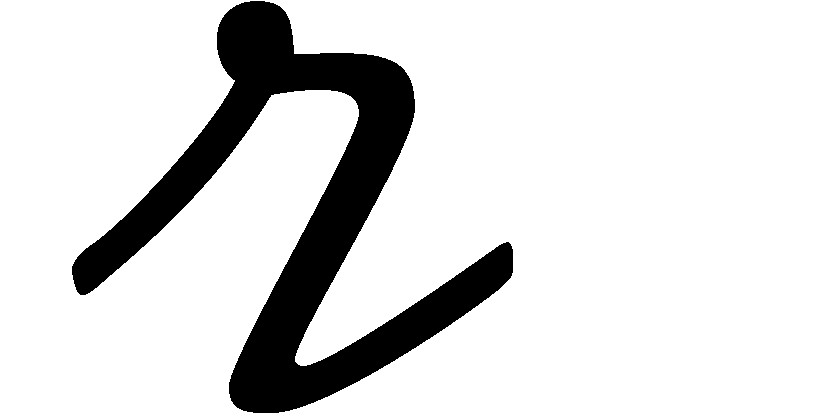
\includegraphics[trim= 1em 0 14em 0,clip]{fonts/ScriptR}}$}}}
\def\brcurs{{\mbox{$\resizebox{.09in}{.08in}{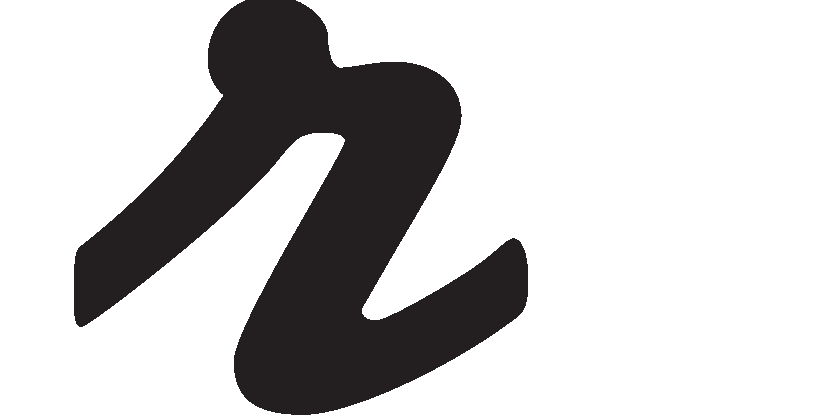
\includegraphics[trim= 1em 0 14em 0,clip]{fonts/BoldR}}$}}}
\def\hrcurs{{\mbox{$\hat \brcurs$}}}


\title{Classical derivation of far-field elastic x-ray scattering under the first Born approximation}
\author{Richard A. Kirian}
\date{\today}

\begin{document}
\maketitle

\section{Overview}

There are multiple ways to develop the theory of x-ray diffraction.  In order to make this guide 
accessible to motivated undergraduates, we will build upon the most popular
undergraduate electrodynamics textbook by David Griffiths\cite{Griffiths2018}.  The main result we derive is
the diffraction intensity equation:
\begin{align}\label{eqn:key}
    I(\vec{q}) = J_0 r_e^2 \Delta \Omega \mathcal{P}(\vec{q})  \abs{\int  
\rho(\vec{r}) e^{-i \vec{q}\cdot\vec{r}} d^3 r }^2 \;.
\end{align}
The above result assumes (1) perfect plane-wave illumination with wavelength $\lambda$, (2) far-field measurements (the
distance to the detector is \emph{much} greater than the size of the object)
and (3) the first-order Born approximation, which loosely means that the scattering amplitudes are very weak
compared to the incident amplitudes. The quantities in equation \ref{eqn:key} are as follows:
\begin{itemize}
\item $I(\vec{q})$ is the x-ray diffraction signal in a pixel (power per 
pixel)
\item $\vec{q}=\vec{k}-\vec{k}_0$ is the wavevector transfer
\item $J_0$ is the incident intensity (power per area)
\item $r_e = 2.818 \times 10^{-15}$~m is the Classical electron radius
\item $\vec{k}_0$ is the incident wavevector with magnitude $|\vec{k}_0| = 
|\vec{k}| = \frac{2\pi}{\lambda}$
\item $\vec{k}$ is the outgoing wavevector that points from the target to the detector pixel
\item $\Delta \Omega$ is the solid angle of the detector pixel (assumed very 
small)
\item $\mathcal{P}(\vec{q})$ is the polarization factor defined below
\item $\rho(\vec{r})$ is the scattering density, which is approximately equal to 
the electron density.
\end{itemize}
%As we can see from equation \ref{eqn:key}, under certain approximations, x-ray diffraction intensities
%allow us to measure the magnitude of the Fourier transform of the scattering density $\rho(\vec{r})$ of the target:
%\begin{align}
%    \abs{F(\vec{q})} \propto \abs{\int  \rho(\vec{r}) e^{-i \vec{q}\cdot\vec{r}} d^3 r } \;.
%\end{align}
%Ideally, we would like to measure the complex \emph{amplitudes} $F(\vec{q})$, in which case
%we could directly recover the scattering density via inverse Fourier transform:
%\begin{align}
%\rho(\vec{r}) = \frac{1}{2\pi} \int  F(\vec{q}) e^{i \vec{q}\cdot\vec{r}} d^3 q \;.
%\end{align}
%The task of recovering the desired molecular structure $\rho(\vec{r})$ given the
%information-deficient
%measurement of $\abs{F(\vec{q})}$ is called the ``phase problem'' in diffraction microscopy and
%crystallography.  The phase problem will be addressed in a separate note.


\section{Electromagnetic fields from a moving point charge}

Here we briefly outline how the electromagnetic 
fields from a moving point charge were derived by Griffiths, starting with Maxwell's equations
in vacuum:
\begin{align}
\nabla \cdot \vec{E} &= \rho/\epsilon_0  &\ \nabla\times\vec{E} &= -\frac{\partial\vec{B}}{\partial t} \\
\nabla \cdot \vec{B} &= 0  & \nabla\times\vec{B} &= \mu_0 \vec{J}+\mu_0 \epsilon_0 \frac{\partial\vec{E}}{\partial t}\;.
\end{align}
As developed in Griffiths chapter 10, Maxwell's equations may be written in terms of the scalar
and vector potentials that are defined as
\begin{align}\label{eqn:pots}
\vec{B} &= \nabla \times \vec{A}\;, & \vec{E} &= -\nabla V -\frac{\partial \vec{A}}{\partial t} \;.
\end{align}
When working in the Lorenz gauge, namely
\begin{align}
\nabla \cdot \vec{A} =  -\mu_0 \epsilon_0 \frac{\partial V}{\partial t} \;,
\end{align}
Maxwell's equations are reduced to a set of four inhomogeneous wave equations:
\begin{align}
\nabla^2 V - \mu_0\epsilon_0 \frac{\partial^2 V}{\partial t^2} &= -\rho / \epsilon_0 & \nabla^2 \vec{A} - \mu_0\epsilon_0 \frac{\partial^2 \vec{A}}{\partial t^2} &= -\mu_0 \vec{J} \;.\label{eqn:ihA}
\end{align}
The inhomogeneous wave equations may be solved using Green's method\footnote{See
Appendix \ref{appendix:inhomogeneous}.}, which yields the retarded potentials:
\begin{align}
V(\vec{r}, t) &= \frac{1}{4\pi\epsilon_0}\int \frac{\rho(\vec{r}', t_r)}{\rcurs}d^3r' & \vec{A}(\vec{r}, t) &= \frac{\mu_0}{4\pi}\int \frac{\vec{J}(\vec{r}', t_r)}{\rcurs}d^3r'
\end{align}
where $\brcurs = \vec{r} - \vec{r}'(t_r)$ and the retarded time is $t_r = t -\rcurs/c$.  For a \emph{point charge} 
moving on the \emph{trajectory} $\vec{r}'(t)$, the retarded potentials become the Li\'enard-Wiechert
potentials\footnote{See Appenxix \ref{appendix:lienard}}:
\begin{align}
V(\vec{r}, t) &= \frac{1}{4\pi\epsilon_0}    \frac{q}{\left| \rcurs - \brcurs \cdot \vec{\beta} \right|} &
\vec{A}(\vec{r}, t) &= \frac{\mu_0}{4\pi}    \frac{q\vec{v}}{\left| \rcurs - \brcurs \cdot \vec{\beta} \right|} \;,
\end{align}
where $\vec{\beta} = \vec{v}/c = \dot{\vec{r}}'(t_r)/c$. From the Li\'enard-Wiechert potentials, Griffiths used equation
\ref{eqn:pots} work out the fields for a point charge:
\begin{align}\label{eqn:Erad}
\vec{E}(\vec{r}, t)= \frac{q}{4\pi\epsilon_0} \frac{\rcurs}{(\brcurs \cdot \vec{u})^3}
[(c^2 - v^2)\vec{u} + \brcurs \times (\vec{u} \times \vec{a})] \; , \quad\quad \vec{B}(\vec{r}, t)
= \frac{1}{c}\hrcurs \times \vec{E}(\vec{r}, t)
\end{align}
where $\vec{u} = c \hrcurs - \vec{\beta}$ and 
$\vec{a}=\ddot{\vec{r}}'(t_r)$.  Importantly, these 
fields are correct for relativistic particles, and as such they may be used to derive both the x-ray scattering
amplitudes as well as the incident source fields created by x-ray free-electron lasers (XFELs) and synchrotrons.


\section{Dipole radiation}

Under the dipole approximations we consider locations very far from a localized 
source.  The electric field contains two terms: the generalized Coulomb field 
and the radiation field:
\begin{align}
\vec{E}(\vec r, t) = \vec{E}_{\text{Coulomb}}(\vec r, t) + \vec 
E_{\text{rad}}(\vec r, t) \;.
\end{align}
The
radiation field in equation \ref{eqn:Erad} dominates because it falls off in proportion to $1/\rcurs$ whereas the generalized
Coulomb field falls off in proportion to $1/\rcurs^2$.  We therefore focus on the
radiation field
\begin{align}
\vec{E}_{\text{rad}}(\vec r, t) = \frac{q}{4\pi\epsilon_0} 
\frac{\rcurs}{(\brcurs\cdot \vec{u})^3}
[\brcurs \times (\vec{u} \times \vec{a})] \; , \quad\quad 
\vec{B}_{\text{rad}}(\vec{r}, t)
= \frac{1}{c}\hrcurs \times \vec{E}(\vec{r}, t)
\end{align}
for the remainder of this note.

Consider a point charge that oscillates about the origin with position $\vec{r}' 
= r_0 \exp(-i\omega t) \hvec{r}'$ (we take the real part of this).
We make the standard dipole radiation assumptions: the dipole is small compared to the distance
to our observation point, which means that $r \gg r'$ and hence $\brcurs \approx \vec{r}$.
We further assume that the charged particle is non-relativistic, which means that\footnote{Equivalently, 
$r_0\omega/c = 2\pi r_0/\lambda \ll 1 $; the wavelength is much
larger than the dipole, and the time it takes light to traverse the extent of the dipole is
small compared to the period of oscillation.}
$v \ll c$, and we may use $\vec{u} \approx c \hrcurs$.  Plugging these in, we get
\begin{align}\label{eqn:dip1}
\vec{E}_{\text{dip}}(\vec{r},t) &= \frac{q}{4\pi\epsilon_0} \frac{r}{(\vec{r}\cdot c \hvec{r})^3}
\vec{r} \times (c \hvec{r} \times \vec{a}) \\
&= \frac{\mu_0 }{4\pi} \frac{1}{r} \hvec{r} \times ( \hvec{r} \times  
\ddot{\vec{p}}(t_r))
\end{align}
where $\vec{p}(t) = q \vec{r}'(t)$ is the dipole moment of the point charge.
The magnetic field is
\begin{align}
\vec{B}_{\text{dip}} =  \frac{1}{c} \hvec{r} \times \vec{E}_{\text{dip}} 
\end{align}
and the Poynting vector is
\begin{align}
\vec{S} =  \frac{1}{\mu_0} \vec{E}_{\text{dip}}\times\vec{B}_{\text{dip}} =  \frac{1}{\mu_0c} E_{\text{dip}}^2\hvec{r} 
= \frac{\mu_0}{16 \pi^2 cr^2} |\hvec{r} \times    \ddot{\vec{p}}|^2\hvec{r} \;.\\
\end{align}
The differential power radiated through a differential area $d\vec{a} = r^2 \sin\theta d\theta d\phi \hvec{r} = r^2 d\Omega \hvec{r}$ is
\begin{align}
dP = \vec{S}\cdot d\vec{a} = \frac{\mu_0 }{16\pi^2 c} |\hvec{r} \times    \ddot{\vec{p}}|^2 d\Omega \; .
\end{align}
The total power radiated away is
\begin{align}
P = \int \frac{dP}{d\Omega} d\Omega =  \frac{\mu_0 }{16\pi^2 c}  \int |\hvec{r} \times    \ddot{\vec{p}}|^2 d\Omega  \; .
\end{align}
The above integral does not depend on the orientation of the coordinate system, and is most easily performed if we choose $|\hvec{r} \times \hvec{p}|^2 = \sin^2\theta$ which yields a factor of $8\pi/3$.  The final result is the Larmor formula:
\begin{align}
P =  \frac{\mu_0 \ddot{p}^2}{6\pi c}  \; .
\end{align}
For sinusoidal oscillations, a time average of the above introduces a factor of $1/2$:
\begin{align}
\avg{dP} &= \frac{\mu_0 \omega^4 p^2}{32\pi^2 c} |\hvec{r}\times\hvec{p}|^2 d\Omega \\
\langle P \rangle &=  \frac{\mu_0 \omega^4 p^2}{12\pi c} \; . \label{eqn:avgpwer}
\end{align}


\section{Thompson scatter from a free electron}

An example of a very simple classical scattering process is a free electron exposed to an electromagnetic wave, which
results in acceleration and hence re-radiation or \emph{scattering}.  Unfortunately, this is not covered in Griffiths.
The force on an electron (mass $m_e$ and charge $e$) due to an incident light beam with oscillating electric field
$\vec{E}_0(t)$ results in the acceleration
\begin{align}
\vec{a}(t) =  -\frac{e}{m_e} \vec{E}_0(t) \;.
\end{align}
If the electron was bound to an atom we could develop a crude model by adding a restoring force and damping force as in Griffiths chapter 9.  In our simple model for a \emph{free} electron, the second derivative of the dipole moment is 
\begin{align} \label{eqn:pddot_thompson}
\ddot{\vec{p}} =  -e \vec{a} = \frac{e^2}{m_e} \vec{E}_0(t) \;.
\end{align}  
Plugging this into the dipole radiation formula \ref{eqn:dip1} gives
\begin{align}
\vec{E}_{\text{dip}} =  -\frac{r_e}{r} [\hvec{r} \times ( \hvec{r} \times  \vec{E}_0(t_r))] 
\end{align}
where we simplified the expression by defining the classical electron radius
\begin{align}
r_e = \frac{1}{4\pi \epsilon_0} \frac{e^2}{m_e c^2} \approx 2.8\times10^{-15} \; {\text{m}} \;.
\end{align}
The Poynting vector is
\begin{align}
\vec{S} =  \frac{1}{\mu_0} \vec{E}_{\text{dip}}\times\vec{B}_{\text{dip}} =  
\frac{1}{\mu_0c} E_{\text{dip}}^2\hvec{r} 
= \frac{\mu_0}{16 \pi^2 cr^2} |\hvec{r} \times    \ddot{\vec{p}}|^2\hvec{r} 
\;.
\end{align}
We therefore have the power captured by a detector pixel:
\begin{align}\label{eqn:dpthompson}
\avg{dP}  = \frac{r_e^2 E_0^2}{ 2 \mu_0 c}  |\hvec{r}\times\hvec{E}_0|^2 d\Omega 
 = I_0 r_e^2  |\hvec{r}\times\hvec{E}_0|^2  d\Omega   \; .
\end{align}
where $I_0 = |\hvec{E}_0|^2/2\mu_0c$ is the incident radiation intensity.  Integrating over all angles we get
\begin{align}
P = \frac{8}{3}\pi r_e^2  I_0  = \sigma_T  I_0 
\end{align}
where $\sigma_T$ is the Thompson scattering cross section.

\section{Polarization Factor}

The ``polarization factor'' is the term $\mathcal{P}=| \hvec{r} 
\times  \hvec{E}_0 |^2=\sin^2\theta$ in equation \ref{eqn:dpthompson}, which
corresponds to linear polarization along the direction $\hvec{E}_0$.  We may 
generalize to an arbitrary elliptical polarization if we write the field as a 
superposition of two orthogonal polarizations:
\begin{align}
 \vec{E}_0 = \vec{E}_1 + e^{i\phi}\vec{E}_2 
\end{align}
where $\hvec{E}_2 = \hvec{k}_0 \times \hvec{E}_1$.  The time-averaged Poynting 
vector becomes\footnote{See Appendix \ref{sec:poynt} for details.}
\begin{align}
\avg{\vec{S}(\vec{r})} &= r_e^2 \frac{1}{r^2} (I_1 | \hvec{r} \times  \hvec{E}_1 
|^2 + I_2 | \hvec{r} \times  \hvec{E}_2 |^2)  \hvec{r} \;. 
\end{align}
If we write the overall incident intensity as 
\begin{align}
 I_0 = I_1 + I_2 
\end{align}
and parameterize the intensity components according to the polarization 
power weight $\alpha$ such that
\begin{align}
 I_1 &=\alpha I_0\\
 I_2 &= (1-\alpha)I_0
\end{align}
we may write the generalization of equation \ref{eqn:dpthompson}:
\begin{align}\label{eqn:genthompson}
\avg{dP} = I_0 r_e^2  (\alpha | \hvec{r} \times  \hvec{E}_1 |^2 + (1-\alpha) 
| \hvec{r} \times  \hvec{E}_2 |^2)  d\Omega\;.
\end{align}
We typically work in terms of the fluence (time-integrated intensity) $J_0$, 
which gives the expression for the measured diffraction signal\footnote{The 
units here are either energy or photons per pixel, depending on the units 
chosen for $J_0$.  Photons are often the preferred unit since the noise 
characteristics often depend on photon counts.}
\begin{align}\label{eqn:keyF}
    I(\vec{q}) = J_0 r_e^2  \mathcal{P}(\vec{q}) \Delta \Omega
\end{align}
where the polarization factor is defined as
\begin{align}\label{eqn:goodpol}
 \mathcal{P}(\vec{q}) = \alpha | \hvec{k} \times  \hvec{E}_1 |^2 + (1-\alpha) | 
\hvec{k} \times \hvec{E}_2 |^2
\end{align}
with the understanding that 
\begin{align}
 \hvec{r} = \hvec{k} = \frac{\vec{q} - \vec{k}_0}{\abs{\vec{q} - \vec{k}_0}} \;.
\end{align}
A convenient form for calculations\footnote{The use of dot products rather 
than angles is preferred since angles are often defined in different ways by 
different textbooks and software packages.  Dot products are invariant to the 
usual coordinate transformations.} is
\begin{align}
 \mathcal{P}(\vec{q}) &= 1 - \alpha(\hvec{k} \cdot \hvec{E}_1 )^2 - 
(1-\alpha)(\hvec{k} \cdot \hvec{E}_2 )^2 \;.
\end{align}



\section{Weak Diffraction (Born approximation)}

Consider the the scattered field from a free electron located at position $\vec{r}'$ under the influence of a plane wave
\begin{align}
 \vec{E}_0(\vec{r},t) = \vec{E}_0 \exp(i\vec{k}_0 \cdot \vec{r} - i \omega t)
\end{align}
The scattered field is
\begin{align}
\vec{E}_{\text{dip}}(\vec{r},t) =  \frac{r_e}{r} [\hvec{r} \times ( \hvec{r} \times  \vec{E}_0 )] \exp(i\vec{k}_0 \cdot \vec{r}' - i \omega t_r)
\end{align}
where $t_r = t - \rcurs/c$.  Since we observe in the ``far-field'', where $r \gg r'$, we may use the following approximation:
\begin{align}
 \rcurs = \sqrt{(\vec{r} - \vec{r}')^2} = \sqrt{r^2 + r'^2 -2\vec{r}\cdot 
\vec{r}'} \approx r  - \hvec{r}\cdot \vec{r}' \;.
\end{align}
Plugging in the approximation $t_r \approx t - r/c + \hvec{r} \cdot \vec r'$ we 
have
\begin{align}
\vec{E}_{\text{dip}}(\vec{r},t) =  \frac{r_e}{r} [\hvec{r} \times ( \hvec{r} \times  \vec{E}_0 )]\exp\left(i\vec{k}_0 \cdot \vec{r}' - i\omega t + i \frac{\omega}{c}( r  - \hvec{r}\cdot \vec{r}')\right) \;.
\end{align}
Defining $\vec{k} = \omega/c\; \hvec{r}=2\pi/\lambda \hvec{r}$ (the outgoing wavevector, directed at the detector) and $\vec{q} = \vec{k}-\vec{k}_0$, we get
\begin{align}
\vec{E}_{\text{dip}}(\vec{r},t) =  r_e\frac{e^{ikr}}{r} e^{-i\omega t}[\hvec{r} \times ( \hvec{r} \times  \vec{E}_0 )]e^{-i\vec{q}\cdot\vec{r}'} \;.
\end{align}
Finally, in order to form a diffraction pattern, we sum over many electrons at positions $\vec{r}_i'$:
\begin{align}
\vec{E}_{\text{diff}}(\vec{r},t) =  r_e\frac{e^{ikr}}{r} e^{-i\omega t}[\hvec{r} \times ( \hvec{r} \times  \vec{E}_0 )] \sum_i e^{-i\vec{q}\cdot\vec{r}_i'} \;.
\end{align}
In the continuum limit, with electron density $\rho(\vec{r})$, we have
\begin{align}
\vec{E}_{\text{diff}}(\vec{r},t) =  r_e\frac{e^{ikr}}{r} e^{-i\omega t}[\hvec{r} \times ( \hvec{r} \times  \vec{E}_0 )] \int \rho(\vec{r}') e^{-i\vec{q}\cdot\vec{r}'} d^3r' \;.
\end{align}
We typically define the ``form factor'' as
\begin{align}\label{eqn:formfactor}
 F(\vec{q}) = \int \rho(\vec{r}') e^{-i\vec{q}\cdot\vec{r}'} d^3r' \;.
\end{align}
This form factor is just the Fourier transform of the electron density, with the conjugate variable $\vec{q}$ being defined by the incoming and outgoing wavevectors.  The time-averaged Poynting vector is\footnote{See Appendix \ref{sec:poynt} for details.}
\begin{align}
\avg{\vec{S}(\vec{r})} = \frac{1}{\mu_0}\avg{
\Re\{\vec{E}_{\text{diff}}\}\times\Re\{\vec{B}_{\text{diff}}\}} = r_e^2 
\frac{1}{r^2} J_0 | \hvec{r} \times  \hvec{E}_0 |^2 \left| \int \rho(\vec{r}') 
e^{-i\vec{q}\cdot\vec{r}'} d^3r' \right|^2 \hvec{r} \;.
\end{align}
Where we have used the incident intensity $J_0 = |\vec{E}_0|^2/2\mu_0c$.  
Assuming a detector pixel with area $d\vec{a} = r^2 d\Omega \hvec{r}$, the power 
into the detector pixel is
\begin{align}
I(\vec{q}) = \avg{\vec{S}(\vec{r})} \cdot d\vec{a} = r_e^2 J_0 | \hvec{r} \times 
 \hvec{E}_0 |^2 \left| \int \rho(\vec{r}') e^{-i\vec{q}\cdot\vec{r}'} d^3r' 
\right|^2 d\Omega\;.
\end{align}
Generalizing the polarization factor yields equation \ref{eqn:key}:
\begin{align}\label{eqn:keyF}
    I(\vec{q}) = J_0 r_e^2  \mathcal{P}(\vec{q})  
\abs{\int \rho(\vec{r}') e^{-i\vec{q}\cdot\vec{r}'} d^3r'}^2 \Delta \Omega \;.
\end{align}
The only difference between a single point-like electron (equation  
\ref{eqn:genthompson}) and a charge distribution (the above equation) is the 
appearance of the form factor $F(\vec{q})$.   


\section{Anomalous Dispersion}

A simple classical model for ``anomalous dispersion'' was developed in 
Griffiths chapter 9, as follows.  Instead of the free electron we considered in 
the previous sections, we allow for a restoring force and a damping force in 
addition to the driving force of the external field.  This model gets us 
closer to one that includes the affects of the atom to which the electrons 
are bound.  The position $\vec{x}$ of the electron obeys the following 
differential equation:
\begin{align}
m_e \frac{d^2\vec{x}}{dt^2} + m_e \gamma \frac{d\vec{x}}{dt} + m_e\omega_0^2 
\vec{x} = e \vec{E}_0 \exp(-i\omega t) \;.
\end{align}
The solution for $\vec{x}(t)$ gives the dipole moment
\begin{align}\label{eqn:dddipole}
\vec{p}(t) = e \vec{x}(t) = \frac{e^2/m_e}{\omega_0^2 - \omega^2 - i \gamma 
\omega}\vec{E}_0 \exp(-i\omega t) \;.
\end{align}
Comparing the above with equation \ref{eqn:pddot_thompson}, we see that the 
correction we should make to the radiation field is
\begin{align}
\vec{E}_{\text{dip}} =  -\frac{\omega^2}{\omega_0^2 - \omega^2 - i \gamma 
\omega}\frac{r_e}{r} [\hvec{r} \times ( \hvec{r} \times  
\vec{E}_0(t_r))] \;
\end{align}
We may call the term involving $\omega$ the ``anomalous dispersion correction''.
Although it is a very simple model, captures many of the basic 
frequency-dependent features of diffraction.  The correction to be made to our 
% previous derivations is to make the following replacement:
% \begin{align}
%     r_e^2 \rightarrow \frac{\omega^4}{(\omega_0^2-\omega^2)^2+\gamma^2 
% \omega^2}r_e^2 \;.
% \end{align}


\section{Atomic Scattering Factors}

When far from resonance, the simplest model for an atomic scattering 
factor is to assume the atom has an
electron density $\rho_n^{(0)}(r)$ and calculate the form factor in equation 
\ref{eqn:formfactor}.  For a rotationally symmetric atom\footnote{Most 
tabulations of scattering factors use a rotational symmetry approximation, and 
it is very rare to image with resolutions that can resolve internal atomic 
structure.} situated at the origin, the atomic scattering factor is defined
as\footnote{Appendix \ref{sec:3d1d} derives \ref{eqn:form}.}
\begin{align}
f_n^{(0)}(q)  = \int_{-\infty}^\infty \rho_n^{(0)}(r) \exp(-i 
\vec{q}\cdot\vec{r}) \; d^3r = \int_0^\infty \rho_n^{(0)}(r)   
\frac{\sin(qr)}{qr}  4\pi r^2 dr \; . \label{eqn:form}
\end{align}
For an atom located at the position $\vec{r}_n$, the scattering factor takes on 
the phase shift
\begin{align}
f_n^{(0)}(\vec{q})  = \int_{-\infty}^\infty \rho_n(|\vec{r}-\vec{r}_n|) \exp(-i 
\vec{q}\cdot\vec{r}) d^3r = f_n^{(0)}(q)
\exp(-i \vec{q}\cdot\vec{r}_n)  \; .
\end{align}
A very common way of accounting for anomalous dispersion in atomic scattering 
factors is to include real and imaginary energy-dependent ``dispersion 
correction'' terms to the scattering factors:
\begin{align}
f_n(q) = f_n^{(0)}(q) + \Delta f_n(E) = f_n^{(0)}(q) + f_n'(E) + i f_n''(E)  \;.
\end{align}
The above three terms can be found in many tabulations in the literature.

For an assembly of atoms, the overall form factor (equivalent to equation 
\ref{eqn:formfactor}) is
\begin{align}
F(\vec{q})  = \sum_n f_n(q)
e^{-i \vec{q}\cdot\vec{r}_n}  \; .
\end{align}
We sometimes define the ``scattering density'' as the inverse 
Fourier transform of the above:
\begin{align}\label{eqn:scatterdens}
\rho(\vec{r})  &= \sum_n^N \rho_n^{(0)}(|\vec{r}-\vec{r}_n|) +  
\delta(\vec{r}-\vec{r}_n) \Delta f_n(E) \; .
\end{align}


% \begin{align}
% I(\vec q) \propto \abs{\int \rho(\vec{r}') 
% e^{-i\vec{q}\cdot\vec{r}'} d^3r'}^2
% \end{align}
% 
% \begin{align}
%  =\abs{F(\vec q)}^2
% \end{align}
% 
% 
% \begin{align}
%  \rho(\vec r) = \frac{1}{(2\pi)^3} \int F(\vec q) e^{i \vec q \cdot \vec r} 
% d^3 q
% \end{align}


\section{Refractive Index}

Starting at equation \ref{eqn:dddipole} and assuming we have a number density 
$N$ of such ``atoms'', the polarization (dipole moment per volume) is
\begin{align}
\vec{P}(t) = N \frac{e^2/m_e}{\omega_0^2 - \omega^2 - i \gamma \omega}\vec{E}_0 
\exp(-i\omega t) \;.
\end{align}
Using the usual definitions for a linear material, $\vec{P} = \epsilon_0 \chi_e 
\vec{E}$, $\epsilon = \epsilon_0 (1+\chi_e)$, and $n = 
\sqrt{\epsilon/\epsilon_0}$, we arrive at the refractive index 
\begin{align}
 n = \sqrt{1+N \frac{e^2/m_e\epsilon_0}{\omega_0^2 - \omega^2 - i 
\gamma \omega}} 
\end{align}
In the high-frequency limit, we have
\begin{align}
 n \approx 1 - \frac{N e^2}{2 m \epsilon_0 \omega^2}  \;.
\end{align}
The above is usually written in terms of the classical electron radius $r_e$:
\begin{align}
 n \approx 1 - \frac{1}{2\pi} r_e N \lambda^2 \;.
\end{align}
Note that the refractive index for x-rays is usually very close to 1, but 
slightly less than 1.  We may relate the index of refraction to the scattering 
density from equation \ref{eqn:scatterdens}:
\begin{align}
 n(\vec{r}) \approx 1 - \frac{1}{2\pi} r_e \rho(\vec{r}) \lambda^2 \;.
\end{align}

% \section{Attenuation}
% 
% The complex wavevector is defined as 
% \begin{align}
%  k = \sqrt{\epsilon\mu_0}\omega
% \end{align}


% Suppose we have a number density $n$ of scatterers with total scattering cross 
% section $\sigma$.  A very thin slab of area $A$ and infinitesimal thickness $dz$ 
% contains $M = n A dz$ particles within the slab.  Suppose a collimated beam of 
% incident intensity $I(z)$ is directed at the slab, and the intensity that exits 
% the other side of the slab is $I(z+dz)$ (assume this intensity is measured far 
% from the slab, where the detector does not detect the scattered light).  The 
% total power radiated away can be equated as
% \begin{align}
% dP = (I(z+dz) - I(z)) A =  -M \sigma A I(z) \;.
% \end{align}
% Re-arranging, we have
% \begin{align}
% \frac{I(z+dz) - I(z)}{I(z)} =  \frac{dI(z)}{I(z)} = -n\sigma dz 
% \end{align}
% Integrating the above, we have 
% \begin{align}
% I(z) =  I(0) e^{- n  \sigma z}  \;.
% \end{align}
% For a dilute suspension of particles the attenuation length is equal to $z_0 = 1/n\sigma$.  For dense suspensions of particles, we need to consider multiple scattering, but this result holds for particles that absorb with cross section $\sigma$.

% \section{Rayleigh scatter from a dielectric sphere}
% 
% Outside of the weak-scattering approximation, diffraction is a complicated 
% process.  There are few exact analytic solutions in such cases.  However, if the 
% object is much smaller than the wavelength of the light, then our dipole 
% approximations can be used, provided that we can determine the relationship 
% between the incident field $\vec{E}_0$ and the dipole that it induces:
% \begin{align}
% \vec{p} = \alpha \vec{E} \;,
% \end{align}
% where $\alpha$ is sometimes referred to as the polarizability of the object.  
% For asymmetric objects, the induced dipole vector will point in a direction that 
% differs from the polarization of the incident field, in which case $\alpha$ 
% would take the form of a $3\times3$ tensor.  
% 
% In Griffiths chapter 4, you considered a dielectric sphere with relative 
% permittivity $\epsilon_r$ placed in a uniform field, and found that the internal 
% field $\vec{E}_0$ within the sphere is 
% \begin{align}
% \vec{E}_{\text{int}} = \frac{3}{\epsilon_r + 2} \vec{E}_0 \;.
% \end{align}
% Assuming that the sphere is much smaller than the wavelength of the radiation, 
% we may use this result to determine the Rayleigh scattering cross section for a 
% dielectric sphere.  The polarization (dipole moment per volume) is 
% $\vec{P}=\epsilon_0\chi_e \vec{E}_{\text{int}} = \epsilon_0(\epsilon_r - 1) 
% \vec{E}_{\text{int}}$, and hence the total dipole moment of a sphere of radius $R$ 
% is
% \begin{align}
% \vec{p} = \frac{4}{3} \pi R^3 \vec{P} = 4 \pi R^3 \epsilon_0  
% \frac{\epsilon_r-1}{\epsilon_r + 2} \vec{E}_0 \;.
% \end{align}
% Next we plug this dipole moment into our differential radiated power (equation 
% \ref{eqn:avgpwer}):
%\begin{align}
%\left\langle \frac{dP}{d\Omega} \right\rangle &= \frac{\mu_0  \epsilon_0^2 
% \omega^4 }{2 c} |\hvec{r}\times\hvec{p}|^2   R^6  
% \left(\frac{\epsilon_r-1}{\epsilon_r + 2}\right)^2 E_0^2 \; .
%\end{align}
%We relate the above to the incident intensity (power per area) $I_0 = 
% \frac{1}{2\mu_0 c} E_0^2$ to get
%\begin{align}
%\left\langle \frac{dP}{d\Omega} \right\rangle &= \frac{\omega^4}{2c^4}  
% |\hvec{r}\times\hvec{p}|^2   R^6  \left(\frac{\epsilon_r-1}{\epsilon_r + 
% 2}\right)^2 I_0 \; .
%\end{align}
%We can integrate over all solid angles to get
% \begin{align}
% P  &= \frac{\omega^4}{2c^4}  \frac{8}{3}\pi   R^6  
% \left(\frac{\epsilon_r-1}{\epsilon_r + 2}\right)^2 I_0 \; .
% \end{align}
% This is the Rayleigh scattering formula, which may be written as
% \begin{align}
% P &= \sigma_R I_0 \;.
% \end{align}
% The total scattering cross section (area units) is often written in terms of 
% the sphere diameter $D$, wavelength $\lambda$, and refractive index $n$:
% \begin{align}
% \sigma_R = \frac{2}{3} \pi^5   \frac{D^6}{\lambda^4}  \left(\frac{n^2-1}{n^2 + 
% 2}\right)^2 \;.
% \end{align}
% There are tons of nanoparticles in the air that scatter light in this way; 
% that's why you can see a bright laser beam in a dark room.  There are also 
% various density fluctuations in the refractive index of materials that are 
% nominally ``homogeneous and isotropic'' -- Rayleigh scattering qualitatively 
% explains why you can also see scattering from a bright laser even in ultrapure 
% water or air.   The blue sky is partly due to the wavelength dependence of 
% Rayleigh scatter; we see more blue light than red because blue scatters more 
% strongly.
%The Rayleigh scattering equation is relevant to my own research because the 
% $\sim$60nm viruses and $\sim$5nm protein molecules that I shoot with x-rays 
% radiate green laser light according to that formula (within reasonable 
% approximation).  I use to determine what optical laser power is needed to see a 
% high-speed beam of biomolecules as they fly into the femtosecond x-ray beam.

\newpage

\appendix

\section{Appendix: Solution to the inhomogeneous wave equation}
\label{appendix:inhomogeneous}

We wish to solve for $V(\vec{r}, t)$ in the inhomogeneous equation
\begin{align}\label{eqn:ihV2}
\nabla^2 V(\vec{r}, t) - \mu_0\epsilon_0 \frac{\partial^2 V(\vec{r}, t)}{\partial t^2} &= -\rho(\vec{r}, t) / \epsilon_0
\end{align}
assuming that we know $\rho(\vec{r}, t)$.  Note that if we solve this 
equation, the same approach may be applied to the components
of the vector potential $\vec{A}$ in equation \ref{eqn:ihA}.

Briefly, Green's method works as follows.  Assume we have a linear operator $\mathcal{L}_{\vec{r}}$ and we 
wish to solve for $V(\vec{r})$ in the following equation:
\begin{align}
 \mathcal{L}_{\vec{r}} V(\vec{r}) = g(\vec{r}) \;.
\end{align}
The $\vec r$ subscript indicates that the operator involves the \emph{unprimed} 
coordinates.
% The fact that the operator is linear means that
% \begin{align}
% \mathcal{L}_{\vec{r}} \big( a V(\vec{r}) + b Q(\vec{r}) \big) =
% a \mathcal{L}_{\vec{r}} V(\vec{r}) + b \mathcal{L}_{\vec{r}} Q(\vec{r})
% \end{align}
% for constants $a$ and $b$.  
Now assume further that we can find the ``Green's function''
$G(\vec{r}, \vec{r}')$ that satisfies the equation
\begin{align}
\mathcal{L}_{\vec{r}} G(\vec{r}, \vec{r}') = \delta(\vec{r}-\vec{r}')
\end{align}
where $\delta(\vec{r}-\vec{r}')$ is the Dirac delta function.  Once equipped with $G(\vec{r}, \vec{r}')$ we may easily
show that the solution for $V(\vec{r})$ is
\begin{align}\label{eqn:useg}
V(\vec{r}) = \int_{\text{Vol}} g(\vec{r}')G(\vec{r}, \vec{r}') d^3 r'\;.
\end{align}
Working the proof backwards from the above, we apply $\mathcal{L}_{\vec{r}}$ to both sides of the equation:
\begin{align}
\mathcal{L}_{\vec{r}} V(\vec{r}) &= \mathcal{L}_{\vec{r}} \int_{\text{Vol}} g(\vec{r}')G(\vec{r}, \vec{r}')d^3 r' \\
&= \int_{\text{Vol}} g(\vec{r}')  \mathcal{L}_{\vec{r}} G(\vec{r}, \vec{r}') d^3 r' \\
    &= \int_{\text{Vol}} g(\vec{r}')  \delta(\vec{r} - \vec{r}') d^3 r' \\
    \mathcal{L}_{\vec{r}} V(\vec{r}) &= g(\vec{r})
\end{align}

In order to solve equation \ref{eqn:ihV2}, we will first remove the time variable by expanding $V(\vec{r})$ and
$\rho(\vec{r})$ into their Fourier transforms:
\begin{align}\label{eqn:Vw}
V(\vec{r}, t) &= \int_{-\infty}^{\infty} V_{\omega}(\vec{r})e^{- i\omega t} d\omega \\
    \rho(\vec{r}, t) &= \int_{-\infty}^{\infty} \rho_{\omega}(\vec{r})e^{- i\omega t} d\omega \;.
\end{align}
We plug the above into equation \ref{eqn:ihV2} we get a differential 
equation for each spectral component:
\begin{align}
(\nabla^2 + k^2) V_\omega(\vec{r}) = -\rho_\omega (\vec{r})/\epsilon_0
\end{align}
where $k = \sqrt{\mu_0\epsilon_0}\omega$.  We now seek the Green's function for
\begin{align}
 (\nabla^2 + k^2)G(\vec{r}, \vec{r}') = \delta(\vec{r}-\vec{r}')
\end{align}
The above is easiest to solve if the delta function is at the origin, so we define $\vec{R} = \vec{r}-\vec{r}'$:
\begin{align}
 (\nabla^2 + k^2)G(\vec{r}, \vec{r}') = \delta(\vec{R})
\end{align}
When written in terms of the $\vec{R}$ coordinates, the RHS is rotationally 
invariant, and hence the Green's function can only be a function of the radial 
magnitude: 
$G(\vec{r}, \vec{r}') = G(R)$.  In writing the Laplacian operator in spherical 
coordinates, we've reduced our equation to a single variable:
\begin{align}\label{eqn:symR}
\left(\frac{1}{R}\frac{\partial}{\partial R}R + k^2\right)G(R) = \delta(R) \;.
\end{align}
If we look in the regions $R \ne 0$ where $\delta(R)=0$ we have the equation
\begin{align}
\frac{\partial}{\partial R}[RG(R)] =- k^2 [R G(R)]  
\end{align}
with the usual solutions
\begin{align}
 G(R) = A \frac{e^{ikR}}{R} + B \frac{e^{-ikR}}{R} \;.
\end{align}
With foresight, we can set $B=0$ because the \emph{incoming} spherical waves produce results
that violate causality (we've effectively introduced a boundary condition at 
infinity).  In order to determine the coefficient $A$ we eliminate the 
Delta function by taking the volume integral of both sides of equation 
\ref{eqn:symR}
about an infinitesimal volume centered on the origin:
\begin{align}
\int_{\text{sphere}}\nabla^2 G(R) d^3R  + k^2 \int_{\text{sphere}} G(R) d^3R = 1 \;.
\end{align}
In the limit $R\rightarrow 0$ we have $G(R) \rightarrow A/R$:
\begin{align}
A \int_{\text{sphere}}\nabla^2 \frac{1}{R} d^3R  + A k^2 \int_{\text{sphere}} \frac{1}{R} 4\pi R^2dR = 1 \;.
\end{align}
For the first term on the LHS we use the result from Griffiths chapter 1: 
 $\nabla^2 (1/R) = -4\pi \delta(R)$.  The second term on the LHS 
vanishes.  Finally giving us
\begin{align}
 A = -\frac{1}{4\pi} \;.
\end{align}
After all the above work, we finally have the Green's function -- an outgoing 
spherical wave:
\begin{align}
 G(\vec{r}, \vec{r}') = - \frac{e^{ik|\vec{r}-\vec{r}'|}}{4\pi 
|\vec{r}-\vec{r}'|} \;.
\end{align}

With the Green's function, we finally plug it into equation \ref{eqn:useg}:
\begin{align}
V_\omega(\vec{r}) = \int_{\text{Vol}} \frac{\rho_\omega(\vec{r}')}{4\pi \epsilon_0} \frac{e^{ik|\vec{r}-\vec{r}'|}}{ |\vec{r}-\vec{r}'|} d^3 r'\;.
\end{align}
Finally, we switch from frequency to the time variable by taking a 
Fourier transform of the above:
\begin{align}
V(\vec{r}, t) &= \int_{-\infty}^\infty \left\{\int_{\text{Vol}} \frac{\rho_\omega(\vec{r}')}{4\pi \epsilon_0} \frac{e^{ik|\vec{r}-\vec{r}'|}}{ |\vec{r}-\vec{r}'|} d^3 r' \right\}e^{-i\omega t}d\omega \\
&=\int_{\text{Vol}} \left\{ \int_{-\infty}^\infty\rho_\omega(\vec{r}') e^{-i\omega (t -|\vec{r}-\vec{r}'|/c)} d\omega\right\}\frac{1}{4\pi \epsilon_0} \frac{1}{ |\vec{r}-\vec{r}'|} d^3 r'  \;.
\end{align}
Comparing the term in the curly braces with equation \ref{eqn:Vw} gives us the 
retarded potential
\begin{align}
V(\vec{r}, t) &= \frac{1}{4\pi\epsilon_0}\int \frac{\rho(\vec{r}', 
t_r)}{\rcurs}d^3r' 
\end{align}
along with the retarded time
\begin{align}
 t_r \equiv t - \rcurs / c \;.
\end{align}


\newpage
\section{Appendix: Li\'enard-Wiechert potential}
\label{appendix:lienard}

We have a particle moving along the trajectory $\vec{w}(t)$, and we want the retarded potential at position $\vec{r}$:
\begin{align}
V(\vec{r}, t) = \frac{1}{4\pi\epsilon_0}\int \frac{\rho(\vec{r}', t_r)}{|\vec{r} - \vec{r}'|} d^3r'
\end{align}
where the retarded time is
\begin{align}
t_r(t, \vec{r}') \equiv t - |\vec{r}-\vec{r}'|/c
\end{align}
The density of a point particle is
\begin{align}
\rho(\vec{r}, t) &= q \delta(\vec{r} - \vec{w}(t)) \\
& = q \int  \delta(\vec{r} - \vec{w}(t')) \delta(t' - t_r(t, \vec{r}'))  dt'
\end{align}
Plug the density into the retarded potential:
\begin{align}
V(\vec{r}, t) = \frac{q}{4\pi\epsilon_0}\iint \frac{  \delta(\vec{r}' - \vec{w}(t')) \delta(t' - t_r(t, \vec{r}'))  }{|\vec{r} - \vec{r}'|} d^3r' dt'
\end{align}
Note that the time $t$ that appears in the retarded time is not the same as the dummy variable $t'$.  Now we do the integral over space, which involves swapping $\vec{r}'$ with $\vec{w}(t)$ everywhere.  In particular, note that there is an 
$\vec{r}'$ in the retarded time $t_r(t, \vec{r}')$
\begin{align}\label{eqn:tint}
V(\vec{r}, t) = \frac{q}{4\pi\epsilon_0}\int \frac{ \delta(t' - t_r(t, \vec{w}(t') )\;)  }{|\vec{r} - \vec{w}(t')|} dt'
\end{align}
Next we need to do the integral over time, but we have a delta function with a function as its argument.  The general rule for a delta function is that it is zero except when the argument is equal to zero.  To handle this situation, we use the 
following general rule:
\begin{align}
\delta(g(x)) &= \frac{\delta(x-x')}{|g'(x')|} 
\end{align}
where $x'$ is implicitly defined by the expression
\begin{align}
g(x') & = 0
\end{align}
and the primed $g'(x)$ means to take the derivative
\begin{align}
g'(x) &\equiv \frac{d }{dx}g(x)  \;.
\end{align}
We therefore can write our delta function in time as:
\begin{align}
\delta(t' - t_r(t, \vec{w}(t') )\;) = \frac{\delta(t' - t^*)}{\left |  \frac{d}{dt'} \left(  t' - \left(t - \frac{|\vec{r} - \vec{w}(t')|}{c}\right) \right)_{t' = t^*} \right |}
\end{align}
We work out the denominator:
\begin{align}
  \frac{d}{dt'} \left(  t' - \left(t - \frac{|\vec{r} - \vec{w}(t')|}{c}\right) \right) &= 1 + \frac{1}{c} \frac{d}{dt'} |\vec{r} - \vec{w}(t')| \\
  &= 1 + \frac{1}{c} \frac{d}{dt'} \left( \left( \vec{r} - \vec{w}(t')\right)^2 \right)^{1/2} \\
  &= 1 + \frac{1}{2c} \frac{1}{ |\vec{r} - \vec{w}(t')| } \frac{d}{dt'}\left( \vec{r} - \vec{w}(t')\right)^2\\
  &= 1 + \frac{1}{2c} \frac{1}{ |\vec{r} - \vec{w}(t')| } \frac{d}{dt'}\left( \vec{r}\cdot \vec{r} + \vec{w}(t')\cdot \vec{w}(t') - 2\vec{r} \cdot \vec{w}(t')\right)\\
&= 1 + \frac{1}{2c} \frac{1}{ |\vec{r} - \vec{w}(t')| } \left( 2 \vec{w}(t')\cdot  \dot{\vec{w}}(t') - 2\vec{r} \cdot 
 \dot{\vec{w}}(t')\right) \\
 &= 1 - \frac{1}{c} \frac{ \left( \vec{r} \cdot 
 \dot{\vec{w}}(t') - \vec{w}(t')\cdot  \dot{\vec{w}}(t') \right)  }{ |\vec{r} - \vec{w}(t')| } \\
 &= 1 - \frac{1}{c} \frac{ \left( \vec{r}  - \vec{w}(t')  \right)\cdot  \dot{\vec{w}}(t') }{ |\vec{r} - \vec{w}(t')| }
\end{align}
We now determine what $t^*$ is by the implicit expression
\begin{align}
t' - \left(t - \frac{|\vec{r} - \vec{w}(t')|}{c}\right) = 0
\end{align}
Compare the above to the definition of the retarded time of the particle:
\begin{align}
t_r = t - \frac{|\vec{r} - \vec{w}(t_r)|}{c}
\end{align}
Thus we have $t^* = t_r$, which we substitute in to get
\begin{align}
V(\vec{r}, t) &= \frac{q}{4\pi\epsilon_0}\int \frac{ 1  }{|\vec{r} - \vec{w}(t')| }\frac{\delta(t' - t_r)}{\left| 1 - \frac{1}{c} \frac{ \left( \vec{r}  - \vec{w}(t')  \right)\cdot  \dot{\vec{w}}(t') }{ |\vec{r} - \vec{w}(t') | } \right|} dt' \\
&= \frac{q}{4\pi\epsilon_0} \frac{ 1  }{|\vec{r} - \vec{w}(t_r)| }      \frac{1}{\left| 1 - \frac{1}{c} \frac{ \left( \vec{r}  - \vec{w}(t_r)  \right)\cdot  \dot{\vec{w}}(t_r) }{ |\vec{r} - \vec{w}(t_r) | } \right|} 
\end{align}
We can now clean this up with the definitions $\dot{\vec{w}}(t_r) = \vec{v}$, $\vec{\beta} = \vec{v}/c$ and $\rcurs = \vec{r} - \vec{w}(t_r)$:
\begin{align}
V(\vec{r}, t) = \frac{1}{4\pi\epsilon_0}    \frac{q}{\left| \rcurs - \brcurs \cdot \vec{\beta} \right|} 
\end{align}
This same procedure may be applied to each of the components of $\vec{A}$ to get
\begin{align}
\vec{A}(\vec{r}, t) = \frac{1}{4\pi\epsilon_0}    \frac{q\vec{v}}{\left| \rcurs - \brcurs \cdot \vec{\beta} \right|} \;.
\end{align}


\section{Appendix: Time-averaged Poynting vector}\label{sec:poynt}

Supposing that we have the electric field $\vec{E}(t)=\vec{E}_0 e^{-i\omega t}$ and corresponding magnetic field $\vec{B}(t)=\vec{B}_0 e^{-i\omega t}=\frac{1}{c} \hvec{k}\times \vec{E}_0e^{-i\omega t}$, and we want the time averaged Poynting vector
\begin{align}
 \avg{\vec{S}} = \frac{1}{T}\int_0^{T}\frac{1}{\mu_0} \Re\{ \vec{E} \}\times \Re\{ \vec{B} \} dt \;,
\end{align}
we must be careful to take the real part of the complex fields.  We can write the real part as
\begin{align}
 \Re\{\vec{E}\} = \frac{1}{2} (\vec{E} + \vec{E}^*)
\end{align}
and plug this into the above:
\begin{align}
 \avg{\vec{S}} = \frac{1}{T}\int_0^{T} \frac{1}{\mu_0}\frac{1}{2} (\vec{E} + \vec{E}^*)\times \frac{1}{2} (\vec{B} + \vec{B}^*) dt \;.
\end{align}
Importantly, the cross terms involving $\vec{E}\times\vec{B}$ and $\vec{E}^*\times\vec{B}^*$ will average to zero because
of the time dependent term $e^{-2i\omega t}$ that remains in the integral.  In the other two terms, there is no time
dependence, and therefore
\begin{align}
 \avg{\vec{S}} = \frac{1}{\mu_0} \frac{1}{4} (\vec{E}\times\vec{B}^* +  \vec{E}^*\times\vec{B}) = \frac{1}{2\mu_0}\Re\{ \vec{E}\times\vec{B}^*\}\;.
\end{align}
In vacuum we have $\vec{B}=\frac{1}{c}\hvec{k}\times \vec{E}$ so that
\begin{align}
 \avg{\vec{S}} = \frac{1}{2c\mu_0}\Re\{ \vec{E}\times(\hvec{k}\times\vec{E}^*)\} = \frac{1}{2c\mu_0} \abs{E}^2 \hvec{k} = I\hvec{k} \;.
\end{align}

If the $E$ field has two orthogonal components $\vec{E}=\vec{E}_1 + \vec{E}_2$ such that $\vec{E}_1\cdot\vec{E}_2=0$ and 
$\vec{B}=\frac{1}{c}\hvec{k}\times \vec{E}$ then
\begin{align}
 \avg{\vec{S}} = \frac{1}{2c\mu_0}\Re\{ (\vec{E}_1 + \vec{E}_2)\times(\hvec{k}\times(\vec{E}_1 + \vec{E}_2)^*)\} \;.
\end{align}
Due to the orthogonality of the field components, the cross terms vanish: e.g.
\begin{align}
 \vec{E}_1 \times(\hvec{k}\times \vec{E}_2^*) = 0 \;.
\end{align}
Therefore the average Poynting vector is
\begin{align}
 \avg{\vec{S}} = \frac{1}{2c\mu_0} ( \abs{\vec{E}_1}^2 + \abs{\vec{E}_2}^2)\hvec{k}\;.
\end{align}

\newpage
\section{Appendix: Fourier transform of rotationally symmetric object}
\label{sec:3d1d}

If we consider just a single atom situated at the origin, the atomic form factor 
is equal to
\begin{align}
 f(\vec{q})  = \int \rho(r) \exp(-i \vec{q}\cdot\vec{r}) \; d^3r \; .
\end{align}
Due to rotational symmetry, we are free to choose a convenient direction 
$\vec{q} = q \hvec{z}$ such that in the
spherical coordinate system we have $\vec{q}\cdot\vec{r} =  q r \cos\theta$.  
Now we write down our Fourier transform with
reference only to the magnitudes $q$ and $r$:
\begin{align}
f(\vec{q})  &= \int_0^{2\pi} d\phi \int_0^\infty \rho(r) r^2 dr \int_0^\pi 
\sin\theta d\theta  \exp(-i q r \cos\theta)\\
&=2\pi \int_0^\infty \rho(r) r^2 dr \int_{-1}^1  d\cos\theta  \exp(-i q r 
\cos\theta)  \\
&=2\pi \int_0^\infty \rho(r) r^2 dr \frac{1}{-iqr}\int_{iqr}^{-iqr}  du  \exp(u) 
 \\
&=2\pi \int_0^\infty \rho(r) r^2 dr \frac{\exp(iqr) - \exp(-iqr)}{iqr}   \\
f(q) &= \int_0^\infty \rho(r)   \frac{\sin(qr)}{qr}  4\pi r^2 dr  
\end{align}

\bibliography{\jobname}
\bibliographystyle{plain}

\end{document}
